%%TITRE
\begin{center}
    \vspace{0.5cm}
    \textbf{\Large JENNRICH'S ALGORITHM - A MATLAB IMPLEMENTATION} \\
    \vspace{0.5cm}
    CHAU Dang Minh
\end{center}

\section{Jennrich's Algorithm}
Let there be a three-order tensor $\X\in\RR^{m\times n\times p}$. Suppose that $\X$ has a canonical polyadic decomposition
\begin{equation}
    \X = [[\mathbf{A}, \mathbf{B}, \mathbf{C}]] = \sum\limits_{i=1}^{r} \mathbf{a}_i\otimes \mathbf{b}_i\otimes \mathbf{c}_i,
\end{equation}

where $\mathbf{A}\in\RR^{m\times r}$, $\mathbf{B}\in\RR^{n\mathbf{C} r}$  and $\mathbf{C}\in\RR^{p\times r}$. Choose a unit vector $\mathbf{x}_i\in\RR^p$ uniformly. We have

\begin{equation}
    \mathbf{M}_x = \sum\limits_{i=1}^{p} a_i\X_{:,:,i} = \sum\limits_{j=1}^{r} \langle \mathbf{c}_j, \mathbf{x} \rangle \mathbf{a}_j\mathbf{b}_j^\top = \mathbf{A}\mathrm{diag}(\langle \mathbf{c}_1, \mathbf{x} \rangle, \ldots, \langle \mathbf{c}_r, \mathbf{x} \rangle) \mathbf{B}^\top.
\end{equation}

Let $\mathbf{D}_x = \mathrm{diag}(\langle \mathbf{c}_1, \mathbf{x} \rangle, \ldots, \langle \mathbf{c}_r, \mathbf{x} \rangle)$ for brevity. We write

\begin{equation}
    \mathbf{M}_x = \mathbf{A} \mathbf{D}_x \mathbf{B}^\top.
\end{equation}

Similarly, we can choose a unit vector $\mathbf{b}$ uniformly and construct the matrix

\begin{equation}
    \mathbf{M}_y = \mathbf{A} \mathbf{D}_y \mathbf{B}^\top.
\end{equation}

If $\mathbf{B}$ is full column rank, we have $\mathbf{B}^\top (\mathbf{B}^\top)^\dag = \mathbf{I}_r$. Therefore,

\begin{equation}
    \mathbf{M}_x\mathbf{M}_y^\dag = \mathbf{A} \mathbf{D}_x \mathbf{B}^\top (\mathbf{B}^\top)^\dag \mathbf{D}_y^\dag \mathbf{A}^\dag = \mathbf{A}(\mathbf{D}_x \mathbf{D}_y^\dag) \mathbf{A}^\dag,
\end{equation}

where $\mathbf{D}_x \mathbf{D}_y^\dag = \mathrm{diag}\left(\dfrac{\langle \mathbf{C}_1, \mathbf{a} \rangle}{\langle \mathbf{C}_1, \mathbf{b} \rangle},\ldots, \dfrac{\langle \mathbf{C}_r, \mathbf{a} \rangle}{\langle \mathbf{C}_r, \mathbf{b} \rangle}\right)$. Since $\mathbf{x}$ and $\mathbf{y}$ are chosen uniformly, the elements of $\mathbf{D}_x \mathbf{D}_y^\dag$ are distinct with probability $1$. Hence, the columns of $\mathbf{A}$ are eigenvectors of $\mathbf{M}_x\mathbf{M}_y^\dag$. Similarly, if $\mathbf{A}$ is full column rank, then

\begin{equation}
    \mathbf{M}_x^\top (\mathbf{M}_y^\top)^\dag = \mathbf{B}(\mathbf{D}_x \mathbf{D}_y^\dag) \mathbf{B}^\dag,
\end{equation}

which means that the columns of $\mathbf{B}$ are eigenvectors of $\mathbf{M}_x^\top (\mathbf{M}_y^\top)^\dag$. Finally, we recover $\mathbf{C}$ using

\begin{equation}
    \X_{(3)} = \mathbf{C}(\mathbf{B}\odot \mathbf{A})^\top.
\end{equation}

\section{Implementation}
Function and class dependencies are given in Figure \ref{fig:jennrich}. We use Alternative Least Square CP to compare the results. Furthermore, the decomposed factors are standardized to unit-normed columns when compose back to a tensor to compare with the original one. If the difference between the original and the reconstructed tensors is less than a tolerance, the algorithm ran successfully. If the rank determined by Jennrich's algorithm is smaller than that by CP and the difference is larger than the tolerance after two run times, Jennrich's algorithm is concluded to be unable to solve such case. Detailed testcases are given in \texttt{testcase\_generator.m}. A sample of testing process is illustrated in Figure \ref{fig:tests}

\begin{figure}[ht]
    \centering
    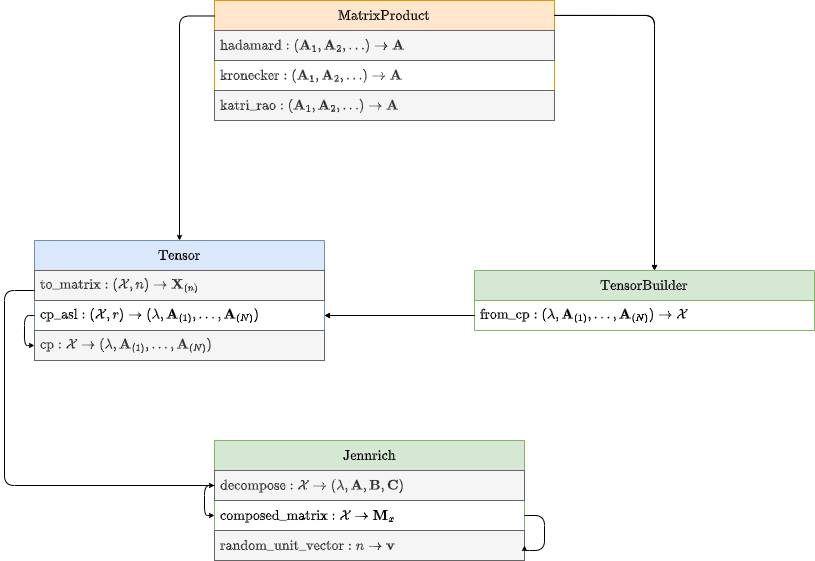
\includegraphics[width=0.8\textwidth]{img/jennrich.png}
    \caption{Jennrich's Algorithm Implementation}
    \label{fig:jennrich}
\end{figure}

\begin{figure}[ht]
    \centering
    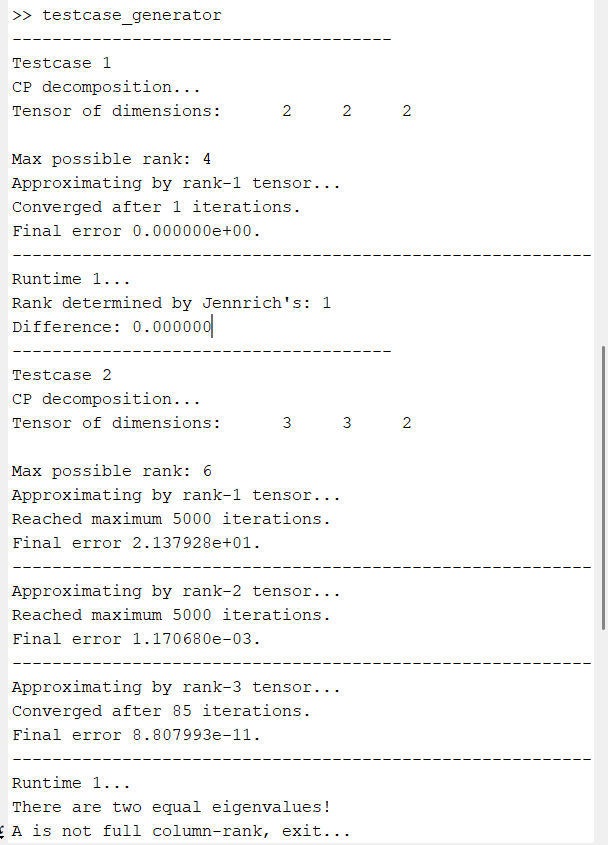
\includegraphics[width=0.8\textwidth]{img/tests.png}
    \caption{Testing}
    \label{fig:tests}
\end{figure}